
\subsection{Embeddings}
Neural networks do not deal well with categorical variables. One hot encoding is a way to handle this. It allows us to represent categorical data as sparse vectors of zeroes and a single 1 representing the specific category. This method has two main drawbacks. Firstly, the dimensionality of the vector representation size grows with the corpus. It can become unmanageable very quick. Secondly, each vector is equidistant from every other vector. This means 'similar' categories are not represented close together in the vector space.

A better way of handling categorical data is through embeddings. When using embeddings we can project categories in a low dimensional latent space and represent them as dense continuous vectors. They are learned parameters and due to this, similar items are projected close together in the latent space. Therefore it is useful in the context of recommendations as we are trying to model user-item similarities. They are also well studied and highly applied in literature for natural language processing to represent words (\citet{embeddings}). Embeddings can be pre-trained and adapted to be used in a model or learned end-to-end with the other parameters.

The main inputs to the model consist of user, item and genre embeddings learned iteratively with the rest of the model parameters.

Genres are handled slightly different than the other two because a movie can have more than one genre. The basis of the embedding is a multi hot encoding, meaning the vector has a value of one for each category that describes it.

\subsection{Activation function}
In a neural network activation functions are mathematical equations, applied to each neuron, that determine if it should activate or not based on its inputs. This function must be computationally efficient to calculate, differentiable and will generally be non-linear. The last part is very important because without non-linearities a NN would just behave like a single-layer perceptron and would not be able to model complex functions. One exception to this is the output layer for a regression NN which will have a linear activation to allow the prediction of any real value.

Early neural networks were using hyperbolic tangent (tanH) and sigmoid activation functions. Sigmoid also known as logistic function is S-shaped and bounded by 1 and 0 \ref{eq:sigmoid}. It suffers from vanishing gradient for very high or low values of x which can result in the network refusing to learn after some point. TanH function is similar to sigmoid but suffers less from the vanishing gradients problem \ref{eq:tanh}.
\begin{equation}
    \label{eq:sigmoid}
    \begin{aligned}
    f(x) &= \frac{1}{1+e^{-x}} \\
    f'(x) &= f(x)(1 - f(x))
    \end{aligned}
\end{equation}

\begin{equation}
    \label{eq:tanh}
    \begin{aligned}
    f(x) &= \frac{2}{1+e^{-2x}} - 1 \\
    f'(x) &= 1 - f(x)^2
    \end{aligned}
\end{equation}

Rectified Linear Unit (ReLU) was first introduced by \citet{relu} in 2010 and is nowadays highly used in deep learning. It introduces sparsity in the network because it outputs 0 for negative numbers \ref{eq:relu}. Moreover, reLU is more computationally efficient than the other two activations. However, a major drawback of using ReLU activations is the "dying ReLU" problem. A ReLU is said to be 'dying' when its stuck outputting 0. The leakyReLU \ref{eq:leakyrelu} is an adaptation of the original. It allows a small value as output for negative samples. This fixes the problem of "dying ReLU" leading to a more robust model (\citet{leakyrelu}).

\begin{equation}
    \label{eq:relu}
    \begin{aligned}
    f(x) &=
    \begin{cases}
        x, & \text{if } x\geq 0 \\
        0, & \text{otherwise}
    \end{cases} \\
    f'(x) &=
    \begin{cases}
        1, & \text{if } x\geq 1 \\
        0, & \text{otherwise}
    \end{cases}
    \end{aligned}
\end{equation}

\begin{equation}
    \label{eq:leakyrelu}
    \begin{aligned}
    f(x) &=
    \begin{cases}
        x, & \text{if } x\geq 0 \\
        0.01x, & \text{otherwise}
    \end{cases} \\
    f'(x) &=
    \begin{cases}
        1, & \text{if } x\geq 1 \\
        0.01, & \text{otherwise}
    \end{cases}
    \end{aligned}
\end{equation}

\begin{figure}[h!]
    \subfloat[Activation functions]{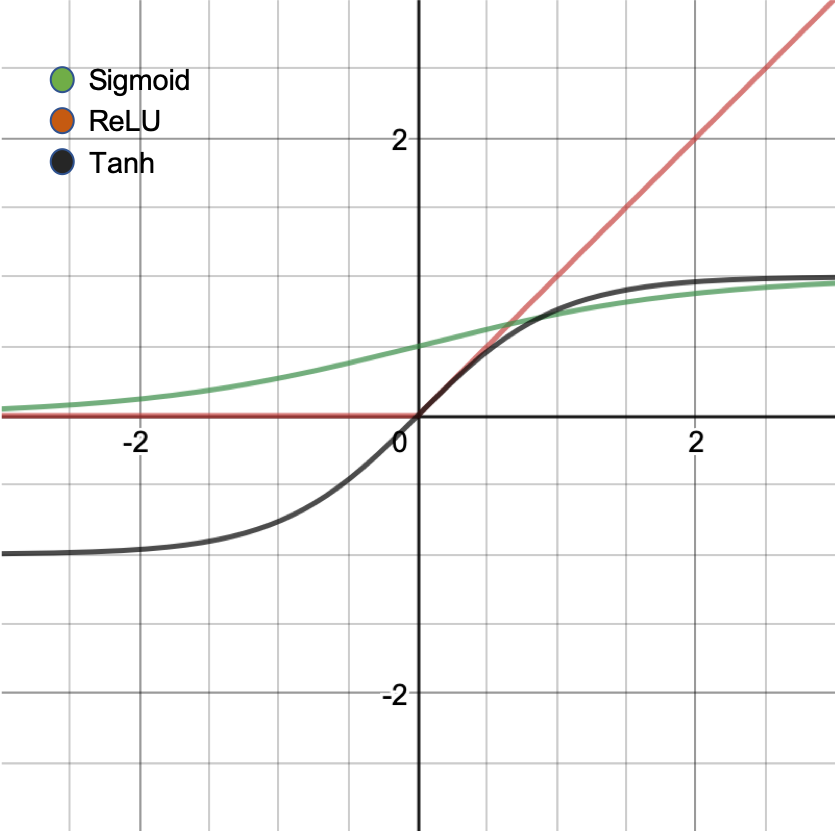
\includegraphics[scale=0.5]{3-activation-func}\label{fig:activations}}
    \hfill
    \subfloat[ReLU vs Leaky ReLU]{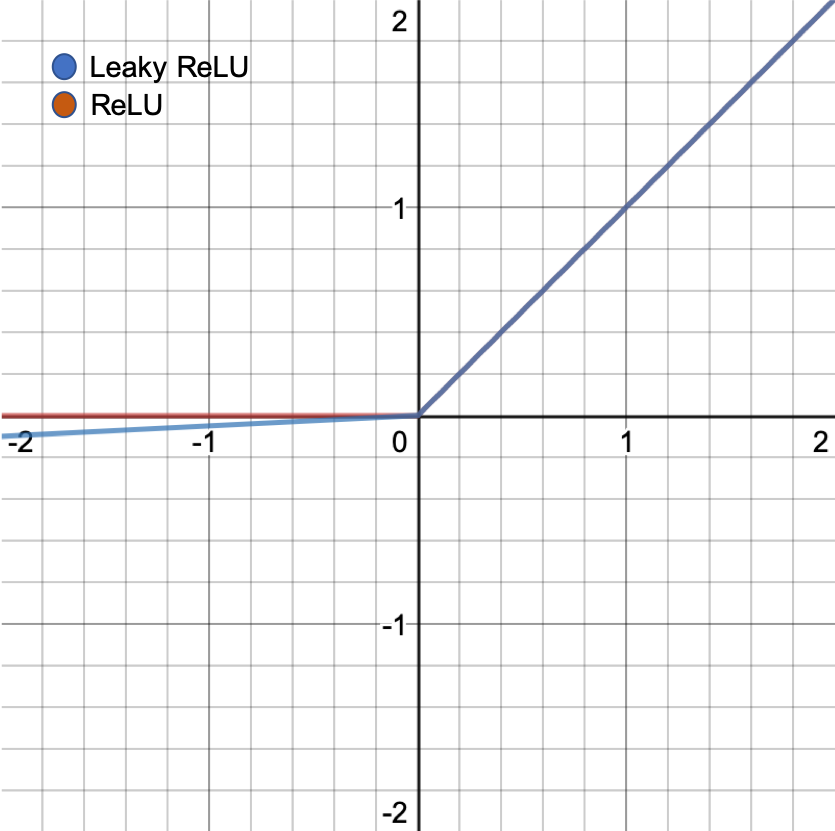
\includegraphics[scale=0.5]{leakyReLUvsReLU}\label{fig:relus}}
\end{figure}


\subsection{Regularization}
One of the most common problems in training neural networks is over-fitting. A model is said to be over-fitting when it performs well on training data but poorly on validation data. Intuitively, it means the model is unable to generalize well and only memorizes the training examples.
This generally occurs if the model is too complex or the size of the training dataset is too small.
Regularization is a method of reducing over-fitting through small modifications of the learning algorithm. The most common types of regularization are l1 and l2. L1 regularization adds the absolute value of the coefficients as penalty term to the cost function. This leads feature sparsity, which is desireable in some cases. L2 is similar but adds the squared value of coefficients as penalty term to the cost function. 

\begin{equation}
    \label{eq:l1l2}
    \begin{aligned}
    l1 penalty = \frac{\lambda}{2m} * \sum{\mid\mid w \mid\mid} \\
    l2 penalty =  \frac{\lambda}{2m} * \sum{\mid\mid w \mid\mid^2}
    \end{aligned}
\end{equation}

In the equations lambda is the hyperparameter controlling the regularization strength. The parameter is usually found using cross-validation or through experimentation. I have experimented with values between \(1e^{-4}\) and \(1e^{-8}\). The final model uses l2 weight regularization on embedding and dense layers with lambda of value \(1e^{-7}\).

Dropout is a special way to regularize the network. This changes the normal training routine by dropping random neurons with a probability p. The edges of a dropped neuron are also removed for that epoch. Therefore, at each epoch we train on a smaller model.
This stops the NN from depending too much on any specific neurons (\citet{dropout}). During testing or prediction phase dropout is disabled. The probability p of dropping neurons is another hyperparameter that has to be selected similar to $\lambda$ in l1 and l2. I have tried values of p between 0.1 - 0.5 in 0.1 increments. The best values of 0.2 and 0.5 are applied in the final model on embedding and dense layers respectively.

\subsection{Optimizer}
Optimizers are a very important parameter in NN configuration. Nowadays there is a vast choice of good optimizers. At its core, an optimizer is an iterative method of optimizing for a cost function. At each optimization step, the weights in the NN will be updated based on the negative of the gradient of the cost function. Stochastic gradient descent (SGD) is a variation of gradient descent in that the optimization happens after each training example. In practice, this usually implies mini-batches of between 32 and 1024 data points (\citet{practical_training}). Batch gradient descent involves updating the weights based on the gradient over the whole dataset. SGD optimizes based on an approximation of the gradient, unlike batch gradient descent. This turns out to be useful as it introduces noise in the network which leads to better generalization. It is also more scalable as the whole dataset does not have to be kept in memory. (\citet{practical_training})

\begin{equation}
    \theta = \theta - \alpha \Delta_{\theta} J(\theta ;x^{(i)}y^{(i)})
\end{equation}

More advanced optimizers are built on top of SGD and include things such as adaptive learning rates and momentum to increase convergence speed and overall stability.

One such algorithm is adaptive moment estimation (Adam). Its widely used in literature and converges much faster than SGD. Adam can be seen as a combination of RMSProp and momentum (\citet{Adam}). Adam uses estimations of first and second order moments of the gradient to adapt the learning rate for each weights in the network.

Nesterov adaptive moment estimation (NAdam) combines adam with nesterov momentum which improve convergence (\citet{NADAM}).

I have decided to use NAdam for training following experiments that proved its the best choice for this specific problem and on this dataset. I am using it with learning rate of $2e^{-4}$, epsilon value of $1e^{-4}$, and the other parameters are keras defaults for this optimizer.

\subsection{Training}
Weight initialization plays an important role in training a neural network. Ideally, we wish the initial weights to be random but not too small and too big, otherwise, it will lead to problems of vanishing or exploding gradients. Xavier normal initialization is one technique that constricts the weights to these characteristics. It works by drawing from a truncated random distribution centered on 0 and with a standard deviation of \(\frac{2}{n_{in} + n_{out}}\), where \(n_{in}\) and \(n_out\) represent the number of inputs and outputs (\citet{initialization}). This is the default initializer used in keras. It is best suited for use in NN that employ tanh activation functions. He normal initialization works better for relu activation. Its similar to xavier, but the standard deviation is \(\frac{2}{n_{in}}\) (\citet{rectifiers}).

\begin{verbatim}
    xavier_w = np.random.rand((n_in, n_out)) * np.sqrt(2 / (n_in + n_out))
    he_w = np.random.rand((n_in, n_out)) * np.sqrt(2 / n_in)
\end{verbatim}

Too speed up the training I have implemented a special generator class extending keras \emph{sequence}. This enables multiprocessing execution of the batch generation algorithm and more importantly it ensures safety and single use of each training example per epoch.
After creating the generator its possible to use the keras \emph{fit\_generator} function with the number of workers and max processing queue size instead of \emph{fit}. This achieves a good speed up in training as the GPU does not have to wait for the CPU to prepare the training batch. More importantly, with these changes it's possible to train on multiple GPUs using data parallelization. In this case the batch will be divided equally among the GPUs. 
Moreover, I have enabled the keras callback \emph{EarlyStopping} with patience of six. This acts as regularization method, because it stop training after the model validation loss has not decreased for 6 consecutive epochs. Moreover, it also rewinds the model parameters to the epoch that had the best loss.

Batch Normalization is a technique proposed by \citet{batchnorm}, which aims to reduce the amount by which hidden unit values shift. It normalizes the input to a layer by subtracting the batch mean and dividing by the batch standard deviation. It turns out this leads to faster convergence and more stability in training. Furthermore, the batch normalization layers also have a small regularization effect which helps the network generalize better.

Finally, the model was trained using 12 workers, a queue size of 200, and batch of 512 data points split evenly between 4 GPUs.

\subsection{Architecture}
The NN architecture follows a common tower pattern, where layers near the top are widest and progressively decrease in width. The inputs to the network consist of user, movie and genre embeddings and average movie and user ratings. They are then concatenated fed into the first hidden layer.
The activation functions employed at the hidden layers are leakyReLU. Each hidden and embedding layer is followed by a dropout layer and a batch normalization layer. The output is made up of a single neuron with linear activation. 

\begin{figure}[h!]
    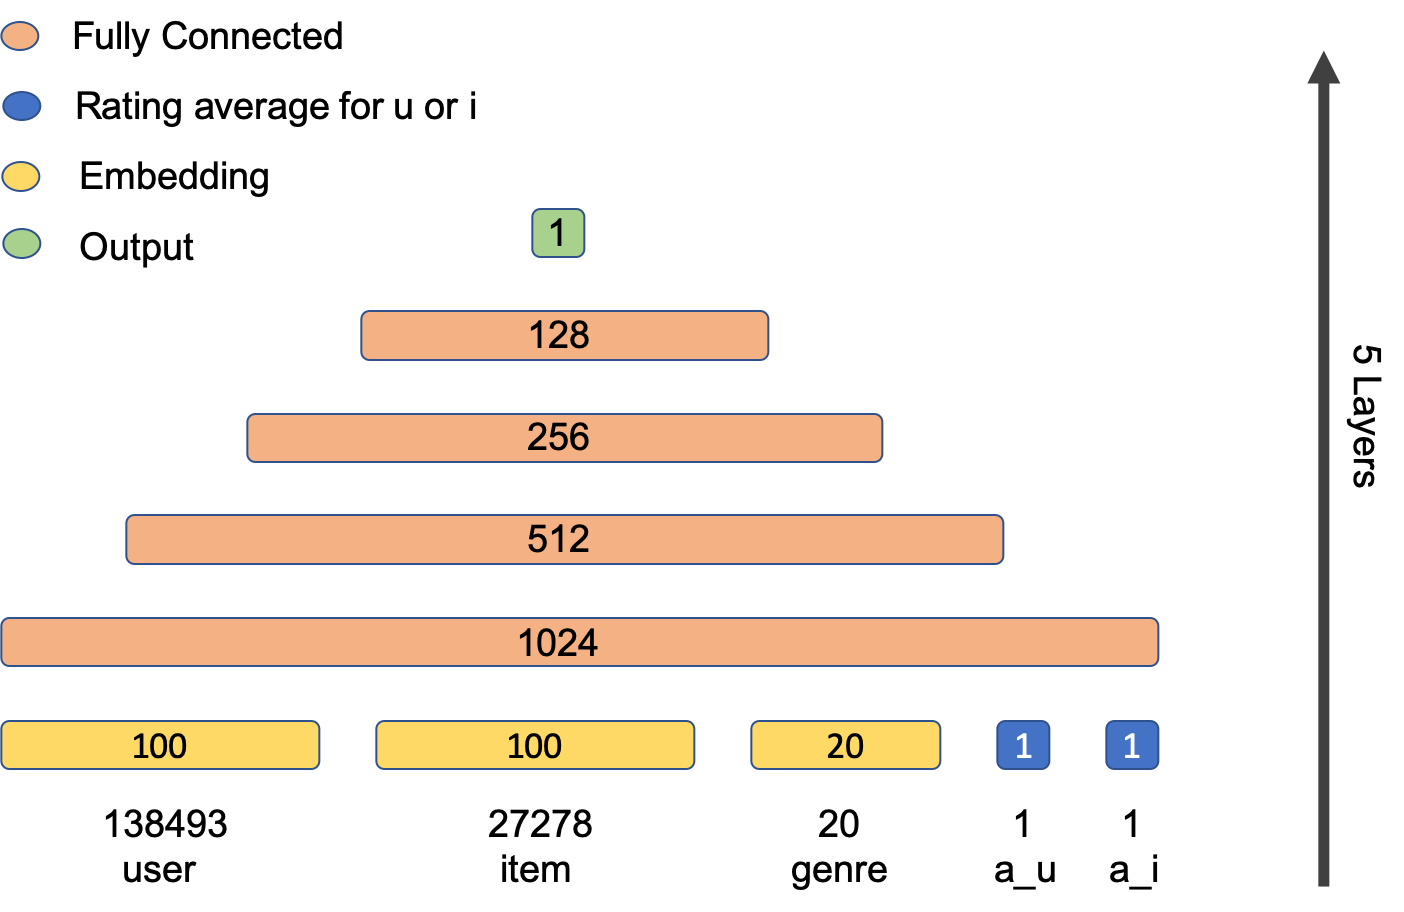
\includegraphics[scale=0.6]{nn_architecture.png}
    \caption{Network architecture}
\end{figure}